\documentclass[11pt]{article}

\usepackage{fullpage}
\usepackage{microtype}

\usepackage{amsmath,amssymb,mathtools,amsthm}
%\usepackage[linesnumbered, ruled]{algorithm2e}
\usepackage[vlined,linesnumbered,ruled]{algorithm2e}
\usepackage{xspace}
\usepackage{paralist}
\usepackage{subcaption}

%\usepackage{color,soul}

%\newcommand{\dror}[1]{\sethlcolor{yellow}\hl{Dror: #1}}

%\usepackage{refcheck}

\renewcommand{\floatpagefraction}{0.8}

\parskip = \smallskipamount

\sloppy

%%%%%%%%%%%%%%%%%%%%%%%%%%%%%%%%%%%%%%%%%%%%%%%%%%%%%%%%%%%%%%%%%

% handy theorems

\newtheorem{lemma}{Lemma}
\newtheorem{observation}[lemma]{Observation}
\newtheorem{theorem}{Theorem}
\newtheorem{definition}{Definition}
\newtheorem{property}{Property}
\newtheorem{corollary}[theorem]{Corollary}
\newtheorem{proposition}{Proposition}

%\spnewtheorem{observation}{Observation}{\bfseries}{\itshape}

%\theoremstyle{plain}
%\newtheorem{observation}[theorem]{Observation}

%%%%%%%%%%%%%%%%%%%%%%%%%%%%%%%%%%%%%%%%%%%%%%%%%%%%%%%%%%%%%%%%%%%%%%%%%

\newcommand{\set}[1]{\left\{ #1 \right\}}
\newcommand{\abs}[1]{\left| #1 \right|}
\newcommand{\ceil}[1]{\left\lceil #1 \right\rceil}
\newcommand{\floor}[1]{\left\lfloor #1 \right\rfloor}
\newcommand{\paren}[1]{\left( #1 \right)}
\newcommand{\eqdf}{\triangleq}
\newcommand{\half}{\frac{1}{2}}
\newcommand{\inv}[1]{\frac{1}{#1}}
\newcommand{\inlineedge}[1]{
\tikz[baseline=-0.5ex, very thick, ->] \draw[#1] (0,0) -- (1,0);
}

\DeclareMathOperator*{\argmin}{arg\,min}
\DeclareMathOperator*{\argmax}{arg\,max}

\def\R{\mathbb{R}}
\def\N{\mathbb{N}}


%%%%%%%%%%%%%%%%%%%%%%%%%%%%%%%%%%%%%%%%%%%%%%%%%%%%%%%%%%%%%%%%%%%%%%%%%

\newcommand{\din}[1][M]{d^{\text{in}}_{#1}}
\newcommand{\dout}[1][M]{d^{\text{out}}_{#1}}
\newcommand{\dinout}[1][M]{d_{#1}}

\newcommand{\nin}[1][M]{N^{\text{in}}_{#1}}
\newcommand{\nout}[1][M]{N^{\text{out}}_{#1}}
\newcommand{\ninout}[1][M]{N_{#1}}

\newcommand{\carpool}{\textsc{Maximum Carpool Matching}\xspace}
\newcommand{\gcp}{\textsc{Maximum Group Carpool Matching}\xspace}

\newcommand{\cmax}{c_{\max}}
\newcommand{\barw}{\bar{w}}
\newcommand{\eps}{\varepsilon}
\newcommand{\inc}{\Gamma}

\newcommand{\calS}{\mathcal{S}}
\newcommand{\calT}{\mathcal{T}}
\newcommand{\calX}{\mathcal{X}}

\newcommand{\calH}{\mathcal{H}}
\newcommand{\calE}{\mathcal{E}}

%%%%%%%%%%%%%%%%%%%%%%%%%%%%%%%%%%%%%%%%%%%%%%%%%%%%%%%%%%%%%%%%%%%%%%%%%

\usepackage{tikz}
\usetikzlibrary{
	arrows.meta,
	calc,
	graphs,
	patterns,
	positioning,
	shapes,
	decorations.pathmorphing,
	math,
}

% NODE
\tikzset{default node/.style={draw,circle,inner sep=0mm,minimum size=5mm,very thick,font=\small,black!70,}}

% LABELS
\tikzset{label/.style={draw=none,sloped,}}
\tikzset{label above/.style={label,midway,above=-1mm,}}
\tikzset{label below/.style={label,midway,below=-1mm,}}

% EDGES
\tikzset{e1/.style={cyan}}
\tikzset{e2/.style={green, loosely dash dot dot}}
\tikzset{e3/.style={blue, loosely dotted}}
\tikzset{e4/.style={loosely dashed}}
\tikzset{e5/.style={red, loosely dashed}}
\tikzset{e6/.style={orange, loosely dash dot}}

% LINES
\tikzset{m/.style={blue, dashed}}
\tikzset{outline/.style={loosely dashed, ultra thin}}

%DEFAULT STYLE
\tikzset{
	>=Triangle[], 
	on grid, 
	auto, 
	thick,
}

%%%%%%%%%%%%%%%%%%%%%%%%%%%%%%%%%%%%%%%%%%%%%%%%%%%%%%%%%%%%%%%%%%%%%%%%%

\begin{document}

\title{%
%
\textbf{Local Search Algorithms for the \\ Maximum Carpool Matching
  Problem}%
%
\thanks{A preliminary version was presented at the 25th Annual
  European Symposium on Algorithms, 2017}
%
}

\author{%
Gilad Kutiel\textsuperscript{*}%
\thanks{Department of Computer Science, Technion, Haifa 32000, Israel.} \\
\texttt{gkutiel@cs.technion.ac.il}\textsuperscript{*}
\and
Dror Rawitz%
\thanks{Faculty of Engineering, Bar Ilan University, Ramat Gan 52900, Israel.
Supported in part by the Israel Science Foundation (grant no.~497/14).} \\
\texttt{dror.rawitz@biu.ac.il}
}

\begin{titlepage}

\maketitle

\begin{abstract}
The \carpool problem is a \emph{star packing} problem in directed
graphs.  Formally, given a directed graph $G = (V, A)$, a capacity
function $c: V \rightarrow \N$, and a weight function $w:
A \rightarrow \R^+$, a \emph{carpool matching} is a subset of arcs,
$M \subseteq A$, such that every $v \in V$ satisfies:%
\begin{inparaenum}[(i)]
\item $\din[M](v) \cdot \dout[M](v) = 0$,
\item $\din[M](v) \leq c(v)$, and 
\item $\dout[M](v) \leq 1$.
\end{inparaenum}
A vertex $v$ for which $\dout[M](v) = 1$ is a \emph{passenger}, and a
vertex for which $\dout[M](v) = 0$ is a \emph{driver} who has
$\din[M](v)$ passengers.  In the \carpool problem the goal is to find
a carpool matching $M$ of maximum total weight.
%
The problem arises when designing an online carpool service, such as
Zimride~\cite{zimride}, which tries to connect between users based on
a similarity function.  The problem is known to be NP-hard, even in
the unweighted and uncapacitated case.
%
The \gcp problem, is an extension of the \carpool where each vertex
represents an unsplittable group of passengers.  Formally, each vertex
$u \in V$ has a size $s(u) \in \N$, and the constraint $\din(v) \leq
c(v)$ is replaced with $\sum_{u:(u,v) \in M} s(u) \leq c(v)$.

We show that \carpool can be formulated as an unconstrained submodular
maximization problem, thus it admits a $\frac{1}{2}$-approximation
algorithm.  We show that the same formulation does not work for \gcp,
nevertheless, we present a local search $(\frac{1}{2}
- \eps)$-approximation algorithm for \gcp.
%
For the unweighted variant of both problems when the maximum possible
capacity, $\cmax$, is bounded by a constant, we provide a local search
$(\half + \inv{2\cmax} - \eps)$-approximation algorithm.  We also
provide an APX-hardness result, even if the maximum degree and $\cmax$
are at most $3$.
\end{abstract}


%\subjclass{F.2.2 Nonnumerical Algorithms and Problems}

\medskip
\noindent
\textbf{Keywords:} approximation algorithms, local search, star
packing, submodular maximization.


\thispagestyle{empty}
\end{titlepage}

%%%%%%%%%%%%%%%%%%%%%%%%%%%%%%%%%%%%%%%%%%%%%%%%%%%%%%%%%%%%%%%%%%%%%%%%%

\section{Introduction}

As traveling costs become higher and parking becomes sparse it is only
natural to share rides or to \emph{carpool}.  Originally, carpooling
was an arrangement among a group of people by which they take turns
driving the others to and from a designated location.  However, taking
turns is not essential, instead passengers can share the cost of the
ride with the driver.  Carpooling has social advantages other than
reducing the costs: it reduces fuel consumption and road congestion
and frees parking space.  
%
While in the past carpooling was usually a fixed arrangement between
friends or neighbors, the emergence of social networks has made
carpooling more dynamic and wide scale.  These days applications like
Zimride~\cite{zimride}, BlaBlaCar~\cite{blablacar},
Moovit~\cite{moovit} and even Waze~\cite{waze} are matching passengers
to drivers.

The matching process of passengers to drivers entails more than
matching the route.
%
Passenger satisfaction also need to be taken into account.  Given
several riding options (including taking their own car), passengers
have preferences.  For example, a passenger may prefer to ride with a
co-worker or a friend.  A passenger may have an opinion on a driver
that she rode with in the past.  She may prefer a non-smoker, someone
who shares her taste in music, or someone who is recommended by
others.
%
Moreover, the matching process may take into account driver
preferences.  For instance, we would like to minimize the extra
distance that a driver has to take.
%
Preferences may also be computed using past information.  Knapen et
al.~\cite{knapen2013estimating} described an automatic service to
match commuting trips.  Users of the service register their personal
profile and a set of periodically recurring trips, and the service
advises registered candidates on how to combine their commuting trips
by carpooling.  The service estimates the probability that a person
$a$ traveling in person's $b$ car will be satisfied by the trip.  This
is done based on personal information and feedback from users on past
rides.

In this paper we assume that potential passenger-driver satisfactions
are given as input and the goal is to compute an assignment of
passengers to drivers so as to maximize the global satisfaction.
%
More formally, we are given a directed graph $G = (V, A)$, where each
vertex $v \in V$ corresponds to a user of the service, and an arc $(u,
v)$ exists if the user corresponding to vertex $u$ is willing to
commute with the user corresponding to vertex $v$.  We are given a
capacity function $c: V \rightarrow \N$ which bounds the number of
passengers each user can drive if she is selected as a driver.  A
non-negative weight function $w : A \rightarrow \R^+$ is used to model
the amount of satisfaction $w(u,v)$ of assigning $u$ to $v$.
%
If $(u,v) \in A$ implies that $(v,u) \in A$ and $w(u,v) = w(v,u)$, the
instance is \emph{undirected}.  If $w(v,u) = 1$, for every $(v,u) \in
A$, then the instance is \emph{unweighted}.  If $c(v) = \deg(v)$, for
every $v$, then the instance is \emph{uncapacitated}.

Given a directed graph $G$ and a subset $M \subseteq A$, define
\(
\din[M](v) \eqdf \abs{\set{u :(u,v) \in M}}
\)
and
\(
\dout[M](v) \eqdf \abs{\set{u :(v,u) \in M}}
%~.
\).
%
A feasible \emph{carpool matching} is a subset of arcs, $M \subseteq
A$, such that every $v \in V$ satisfies:%
\begin{inparaenum}[(i)]
\item $\din[M](v) \cdot \dout[M](v) = 0$,
\item $\din[M](v) \leq c(v)$, and 
\item $\dout[M](v) \leq 1$.
\end{inparaenum}
A feasible carpool matching $M$ partitions $V$ as follows:
\begin{align*}
P_M & \eqdf \set{v : \dout[M](v) = 1} \\
D_M & \eqdf \set{v : \din[M](v) \geq 1} \\
Z_M & \eqdf \set{v : \dout[M](v) = \din[M](c) = 0}
%~,
\end{align*}
where $P_M$ is the set of \emph{passengers}, $D_M$ is the set of
\emph{active drivers}, and $Z_M$ is the set of \emph{solo drivers}.
%
In the \carpool problem the goal is to find a matching $M$ of maximum
total weight, namely to maximize $w(M) \eqdf \sum_{(v,u) \in M}
w(v,u)$.  In other words, the \carpool problem is about finding a set
of (directed toward the center) vertex disjoint stars that maximizes
the total weight of the arcs.  
%
Figure~\ref{fig:carpool} contains an example of a \carpool instance.
%
Note that in the unweighted case the goal is to find a carpool
matching $M$ that maximizes $\abs{P_M}$.
%
Moreover, observe that if $G$ is undirected, $D_M \cup Z_M$ is
a \emph{dominating set}.  Hence, in this case, an optimal carpool
matching induces an optimal dominating set and vice versa.
Since \textsc{Minimum Dominating Set} is NP-hard, it follows
that \carpool is NP-hard even if the instance is undirected,
unweigthed, and uncapacitated.

\begin{figure}[t]
\centering
\newcommand{\edge}[3]{
	\draw (#1) -- (#2) node[label above] {#3};
}

\begin{subfigure}[t]{.45\linewidth}
\centering
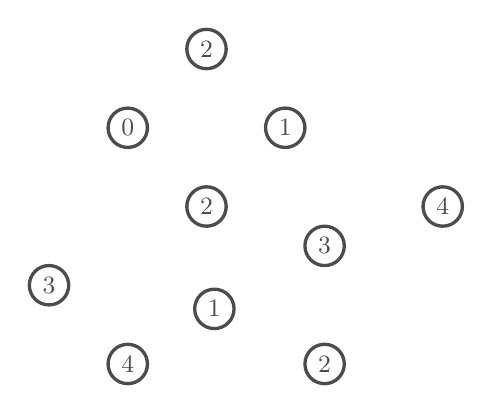
\begin{tikzpicture}[every node/.style={default node}, ->, very thick]

\node(1) at(-1,3) {2};
\node(2) at(.5,.5) {3};
\node(3) at(-.9,-.3) {1};
\node(4) at(-1,1) {2};
\node(5) at(-2,2) {0};
\node(6) at(-2,-1) {4};
\node(7) at(-3,0) {3};
\node(8) at(.5,-1) {2};
\node(9) at(0,2) {1};
\node(10) at(2,1) {4};

\edge{1}{4}{3}
\edge{2}{4}{4}
\edge{3}{4}{5}

\edge{5}{7}{2}
\edge{6}{7}{4}

\edge{8}{10}{6}
\edge{9}{10}{2}

\edge{1}{5}{4}
\edge{4}{5}{4}

\edge{2}{3}{2}
\edge{6}{3}{2}
\edge{7}{3}{2}

\edge{8}{2}{1}
\edge{10}{2}{1}

\edge{3}{8}{3}
\edge{8}{3}{3}

\edge{1}{9}{1}
\edge{4}{9}{1}

\end{tikzpicture}
\caption{An instance containing a directed graph with capacities on
  the vertices and weights on the arcs. }
\end{subfigure}
%
\hfill
%
\begin{subfigure}[t]{.45\linewidth}
\centering
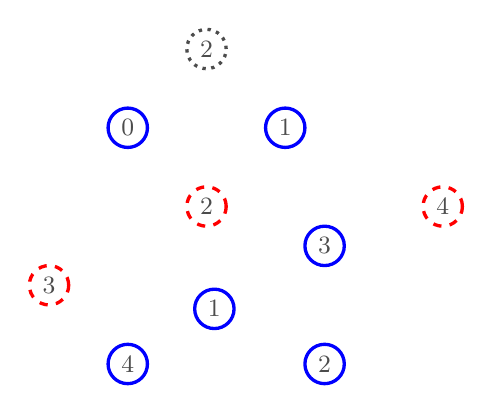
\begin{tikzpicture}[every node/.style={default node}, ->, very thick]

\node[dotted](1) at(-1,3) {2};

\begin{scope}[every node/.style={default node, draw=blue}]
\node(5) at(-2,2) {0};
\node(6) at(-2,-1) {4};

\node(2) at(.5,.5) {3};
\node(3) at(-.9,-.3) {1};

\node(8) at(.5,-1) {2};
\node(9) at(0,2) {1};
\end{scope}

\begin{scope}[every node/.style={default node, draw=red, dashed}]
\node(7) at(-3,0) {3};

\node(4) at(-1,1) {2};

\node(10) at(2,1) {4};
\end{scope}


\edge{2}{4}{4}
\edge{3}{4}{5}

\edge{5}{7}{2}
\edge{6}{7}{4}

\edge{8}{10}{6}
\edge{9}{10}{2}

\end{tikzpicture}
\caption{A feasible carpool matching with total weight of 23.  $P_M$
  is the set of blue, solid vertices, and $D_M$ is the set of red,
  dashed vertices, and $Z_M$ contains only the dotted, black vertex.}
\end{subfigure}
\caption[]{
\label{fig:carpool}
A \carpool example.
%(\subref{carpool:input}) an instance containing a
%directed graph with capacities on the vertices and weights on the
%arcs.  (\subref{carpool:output}) a feasible matching with total weight
%of 23.  $P_M$ is the set of blue vertices, and $D_M$ is the set of
%red, dashed vertices, and $Z_M$ contains only the dotted, black
%vertex.
}
\end{figure}  

%In this paper
%
We also consider an extension of \carpool, called \gcp, in which each
vertex represents a group of passengers, and each group may have a
different size.  Such a group may represent a family or two friends
traveling together.  Formally, each vertex $u \in V$ has a size
$s(u) \in \N$, and the constraint $\din[M](v) \leq c(v)$ is replaced
with the constraint $\sum_{u:(u,v) \in M} s(u) \leq c(v)$.
%
Notice that \textsc{Knapsack} is the special case where only arcs
directed at a single vertex have non-zero (integral) weights.

%%%%%

\paragraph*{Related work.}
%
Agatz et al.~\cite{agatz2012optimization} outlined the optimization
challenges that arise when developing technology to support
ride-sharing and survey the related operations research models in the
academic literature.
%
Hartman et al.~\cite{hartman2014theory} designed several heuristic
algorithms for the \carpool problem and compared their performance on
real data.  Other heuristic algorithms were developed by Knapen et
al.~\cite{knapen2014exploiting}.
%
Hartman~\cite{hartman2013optimal} proved that the \carpool problem is
NP-hard even in the case where the weight function is binary and
$c(v) \leq 2$ for every $v \in V$.  In addition, Hartman presented a
natural integer linear program and showed that if the set of drivers
is known, then an optimal assignment of passengers to drivers can be
found in polynomial time using a reduction to \textsc{Network Flow}
(see also~\cite{kutiel2017}.)
%
Kutiel~\cite{kutiel2017} presented a $\frac{1}{3}$-approximation
algorithm for \carpool that is based on a \textsc{Minimum Cost Flow}
computation and a local search $\half$-approximation algorithm for the
unweighted variant of \carpool.  The latter starts with an empty
matching and tries to improve the matching by turning a single
passenger into a driver.

Nguyen et al.~\cite{nguyen2008approximating} considered the
\textsc{Spanning Star Forest} problem.  A \emph{star forest} is a
graph consisting of vertex-disjoint star graphs.  In the
\textsc{Spanning Star Forest} problem, we are given an undirected
graph $G$, and the goal is to find a spanning subgraph which is a star
forest that maximizes the weight of edges that are covered by the star
forest.  Notice that this problem is equivalent to \carpool on
undirected and uncapacitated instances.  We also note that if all
weights leaving a vertex are the same, then the instance is referred
to as vertex-weighted.
%
Nguyen et al.~\cite{nguyen2008approximating} provided a PTAS for
unweighted planner graphs and a polynomial-time
$\frac{3}{5}$-approximation algorithm for unweighted graphs.  They
gave an exact optimization algorithm for weighted trees, and used it
on a maximum spanning tree of the input graph to obtain a
$\frac{1}{2}$-approximation algorithm for weighted graphs.  They also
shows that it is NP-hard to approximate unweighted \textsc{Spanning
Star Forest} within a ratio of $\frac{259}{260}+\eps$, for any
$\eps>0$.
%
%They also showed how to apply the spanning star forest model to
%aligning multiple genomic sequences over a tandem duplication region.
%
Chen et al.~\cite{CENRRS13} improved the approximation ratio for
unweighted graphs from $\frac{3}{5}$ to $0.71$ and gave a
$0.64$-approximation algorithm for vertex weighted graphs.  They also
showed that the edge- and vertex-weighted problem cannot be
approximated to within a factor of $\frac{19}{20} + \eps$, and
$\frac{31}{32} + \eps$, resp., for any $\eps > 0$, assuming that
$\text{P} \neq \text{NP}$.
%
Chakrabarty and Goel~\cite{ChakrabartyGoel10} improved the lower bounds
to $\frac{10}{11} + \eps$ and $\frac{13}{14}$.

Athanassopoulos et al.~\cite{ACKK09} improved the ratio for the
unweighted case to $\frac{193}{240} \approx 0.804$.
%
They considered a natural family of \emph{local search} algorithms for
\textsc{Spanning Star Forest}.  Such an algorithm starts with the
solution where all vertices are star centers.  Then, it repeatedly
tries to turn $t \leq k$ from leaves to centers and $t+1$ centers to
leaves.  A change is made if it results in a feasible solution, namely
if each leave is adjacent to at least one center.  The algorithm
terminates when such changes are no longer possible.
%
Athanassopoulos et al.~\cite{ACKK09} showed that, for any $k$ and
$\eps \in (0,\inv{2(k+2)}]$, there exists an instance $G$ and a local
optima whose size is smaller than $(\half + \eps) \textsc{opt}$,
where \textsc{opt} is the size of the optimal spanning star forest.
We note that, for a given $k$, the construction of the above result
requires that the maximum degree of $G$ is at least $2(k+2)$.  Hence,
this result does not hold in graphs with maximum degree $\Delta$.

Arkin et al.~\cite{arkin2004approximations} considered
the \textsc{Maximum Capacitated Star Packing} problem.  In this
problem the input consists of a complete undirected graph with
non-negative edge weights and a capacity vector $c
= \set{c_1,\ldots,c_p}$, where $\sum_{i=1}^p c_i = \abs{V} - p$.  The
goal is to find a set of vertex-disjoint stars in $G$ of size
$c_1,\ldots,c_p$ of maximum total weight.  Arkin et
al.~\cite{arkin2004approximations} provided a local search algorithm
whose approximation ratio is $\inv{3}$, and a matching-based
$\half$-approximation algorithm for the case where edge weights
satisfy the triangle inequality.

Bar-Noy et al.~\cite{bar2015improved} considered the
\textsc{Minimum $2$-Path Partition} problem.
In this problem the input is a complete graph on $3k$ vertices with
non-negative edge weights, and the goal is to partition the graph into
disjoint paths of length 2.  This problem is the special case of the
undirected carpool matching where $c(v) = 2$, for every $v \in V$.
They presented two approximation algorithms, one for the weighted case
whose ratio is $0.5833$, and another for the unweighted case whose
ratio is $\frac{3}{4}$.

Another related problem is \textsc{$k$-Set Packing}, where one is
given a collection of weighted sets, each containing at most $k$
elements, and the goal is to find a maximum weight subcollection of
disjoint sets.  Chandra and Halld\'orsson~\cite{chandra2001greedy}
presented a $\frac{3}{2(k+1)}$-approximation algorithm for this
problem, and Berman~\cite{Berman00} gave a
$\frac{2}{k+1}$-approximation algorithm.
%
\carpool can be seen as a special case of \textsc{$k$-Set Packing}
with $k = \cmax + 1$.  Consider a subset of vertice $U$ of size at
most $k$.  Observe that each subset of vertices has an optimal
internal assignment of passenger to drivers.  Let the weight of this
assignment be the profit of $U$, denote by $p(U)$.  If $k = O(1)$,
$p(U)$ can be computed for every $U$ of size at most $k$ in polynomial
time.  The outcome is a \textsc{$k$-Set Packing} instance.  This leads
to a $\frac{2}{\cmax+2}$-approximation algorithm for \carpool for the
case where $\cmax = O(1)$.


%%%%%

\paragraph*{Our contribution.}
%
Section~\ref{sec:approx} contains approximation algorithms for
\carpool.  First, in Section~\ref{sec:sub} we show that \carpool can
be formulated as an unconstrained submodular maximization problem,
thus it has a $\frac{1}{2}$-approximation algorithm due
to~\cite{BFNS15,buchbinder2016deterministic}.  On the other hand, we
show that the unconstrained submodular maximization formulation for
\carpool does not work for \gcp.
%
We present a local search algorithm for \carpool which repeatedly
checks whether the current carpool matching can be improved by means
of a star centered at a vertex, and it terminates when such a step is
not possible.
%
The approximation ratio of this algorithm is $\half$ if weights are
polynomially bounded, and its ratio is $\half-\eps$ in general.  This
algorithm extends to \gcp with the same approximation ratio.
%We show, however, that this problem still
%admits a $(\frac{1}{2} -\varepsilon)$-approximation algorithm by
%extending our first local search algorithm.

In Section~\ref{sec:cmax} we consider \carpool with bounded maximum
capacity.   
%
In Section~\ref{sec:hardness} we show that \carpool is APX-hard even
for undirected and unweighted instances with $\Delta \leq b$, for any
$b \geq 3$.
%
In Section~\ref{sec:local} we provide another local search algorithm,
whose approximation ratio is $\half + \inv{2\cmax} - \eps$, for any
$\eps>0$, for unweighted \carpool, where $\cmax \eqdf \max_{v \in V}
c(v)$.  Given a parameter $k$, our algorithm starts with the empty
carpool matching.  Then, it repeatedly tries to find a better matching
by replacing $t \leq k$ arcs in the current solution by $t+1$ arcs
that are not in the solution.
%
%We show that our analysis is tight.
%
We also note that our algorithm falls within the local search family
defined in~\cite{ACKK09}.  However, on undirected and uncapaciated
instances we have that $\cmax = \Delta$, and as mentioned above the
result from~\cite{ACKK09} does not hold in bounded degree graphs.
%
In addition, we show that our local search algorithm generalizes to
unweighted \gcp with the same approximation ratio.

%%%%%%%%%%%%%%%%%%%%%%%%%%%%%%%%%%%%%%%%%%%%%%%%%%%%%%%%%%%%%%%%%%%%%%%%%

\section{Approximation Algorithms}
\label{sec:approx}

We present two algorithms for \carpool: a $\frac{1}{2}$-approximation
algorithm that is based on formulating the problem as an unconstrained
submodular maximization problem and a local search $(\frac{1}{2} -
\varepsilon)$-approximation algorithm.  While the latter does not
improve upon the former, it will be shown
%(in Section~\ref{sec:group})
that it can be generalized to \gcp without decreasing the
approximation ratio.

%%%%% 

\subsection{Submodular Maximization}
\label{sec:sub}

In this section we show that the \carpool problem can be formulated as
an unconstrained submodular maximization problem, and thus it has a
$\frac{1}{2}$-approximation algorithm due to Buchbinder et
al.~\cite{BFNS15,buchbinder2016deterministic}.

Given a \carpool instance $(G = (V,A), c, w)$, consider a subset
$S \subseteq V$.  Let $M(S)$ be a maximum weight carpool matching
satisfying $D_{M(S)} \subseteq S \subseteq V \setminus P_{M(S)}$,
namely $M(S)$ is the best carpool matching whose drivers belong to $S$
and whose passengers belong to $V \setminus S$.  In other words,
$M(S)$ is the maximum weight carpool matching that is a subset of
$A \cap (V \setminus S) \times S$.
%
Given $S$, the carpool matching $M(S)$ can be computed in polynomial
time by computing a maximum $b$-matching in the bipartite graph $B =
(V \setminus S, S, A \cap (V \setminus S) \times S)$ which can be done
using an algorithm for \textsc{Minimum Cost Flow} as shown
in~\cite{kutiel2017}.

Consider the function $\barw: 2^V \to \R$, where
\[
\barw(S) \eqdf w(M(S)) = \sum_{e \in M(S)} w(e)
~.
\]
Observe that $\barw(\emptyset) = \barw(V) = 0$, and that $\barw$ is
not monotone.
%
In the next lemma we prove that $\bar{w}$ is a \emph{submodular set
function}.  Recall that a function $f$ is submodular if $f(S) +
f(T) \geq f(S \cup T) + f(S \cap T)$ for every two sets $S$ and $T$ in
the domain of $f$.

\begin{lemma}
$\barw$ is submodular.
\end{lemma}
\begin{proof}
Consider any two subsets $S, T \subseteq V$.  We show that $\barw(S)
+ \barw(T) \geq \barw(S \cup T) + \barw(S \cap T)$.
%
Let $M(S \cup T)$ and $M(S \cap T)$ be optimal carpool matchings with
respect to $S \cup T$ and $S \cap T$.
%
To prove the lemma we construct two feasible carpool matchings $M_S$
and $M_T$ such that $M_S \subseteq (V \setminus S) \times S$, $M_T
\subseteq (V \setminus T) \times T$, and $M_S \cup M_T = M(S \cup T)
\biguplus M(S \cap T)$, where the RHS can be a multiset.
%
The lemma follows, since $\barw(S) \geq w(M_S)$ and $\barw(T) \geq
w(M_T)$.

First, add all the edges in $M(S \cup T)$ entering $S \setminus T$ to
$M_S$.  Similarly, add all the edges in $M(S \cup T)$ entering
$T \setminus S$ to $M_T$.  Observe that $\din[M_S](v) = \din[M(S \cup
T)](v) \leq c(v)$, for every $v \in S \setminus T$ and that
$\din[M_T](v) = \din[M(S \cup T)](v) \leq c(v)$, for every $v \in
T \setminus S$.
%
Next, add the edges in $M(S \cap T)$ leaving $T \setminus S$ to $S$
and add the edges in $M(S \cap T)$ leaving $S \setminus T$ to $T$.
%
It remains to distribute the edges leaving $V \setminus (S \cup T)$
and entering $S \cap T$ in both $M(S \cup T)$ and $M(S \cap T)$.  Note
that there may exist edges $(v,u)$, where $v \not\in S \cup T$, and $u
\in S \cap T$ such that $(v,u) \in M(S \cup T)$ and $(v,u) \in M(S
\cap T)$.  We refer to this edges as \emph{duplicate} edges.
%
We add all edges leaving $V \setminus (S \cup T)$ and entering $S \cap
T$ in $M(S \cap T)$ to $M_S$.  Notice that this is possible, since
after this addition we have that $\din[M_S](v) \leq \din[M(S \cap
T)](v) \leq c(v)$, for every vertex $v \in S \cap T$.
%
Then we add all duplicate edges in $M(S \cup T)$ to $M_T$.
%
The remaining edges are distributed between $M_S$ and $M_T$ without
violating capacities.  This can be done, since $\din[M(S \cup T)](v)
+ \din[M(S \cap T)](v) \leq 2c(v)$, for every $v \in S \cap T$.
%
Figure~\ref{fig:sub} contains a graphical representation of the above
edge distribution.
\end{proof}

\begin{figure}[t]
\centering
\def \sst {\draw[e1] (-2, -.5) -- (-.5, -.5);}
\def \tst {\draw[e2] (2, -.5) -- (.5, -.5);}

\def \os {\draw[e3] (-2, 1.5) -- (-2, .4);}
\def \cupst {\draw[e4] (-.5, 1.5) -- (-.5, .4);}
\def \capst {\draw[e5] (.5, 1.5) -- (.5, .4);}
\def \ot {\draw[e6] (2, 1.5) -- (2, .4);}

\begin{subfigure}{.48\linewidth}
\centering
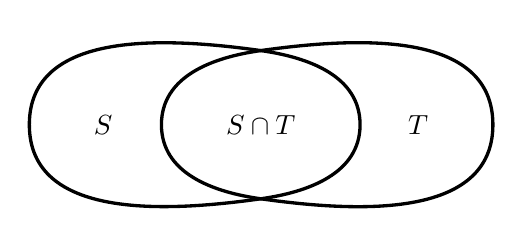
\begin{tikzpicture}[very thick]

\begin{scope}[every node/.style={inner sep=.8cm}]
\node(s) at(-2,0) {$S$};
\node(st) at(0,0) {$S \cap T$};
\node(t) at(2,0) {$T$};
\end{scope}

\draw 
(s.west) to[out=90, in=172] 
(st.north) to[out=-8, in=90] 
(st.east) to[out=270, in=8]
(st.south) to[out=188, in=270]
(s.west)
;

\draw 
(t.east) to[out=90, in=8] 
(st.north) to[out=188, in=90] 
(st.west) to[out=270, in=172]
(st.south) to[out=-8, in=270]
(t.east)
;

\begin{scope}[->]
\os
\cupst
\ot
\end{scope}

\end{tikzpicture}
\caption{}
\label{sub:cup}
\end{subfigure}
%
\hfill
%
\begin{subfigure}{.48\linewidth}
\centering
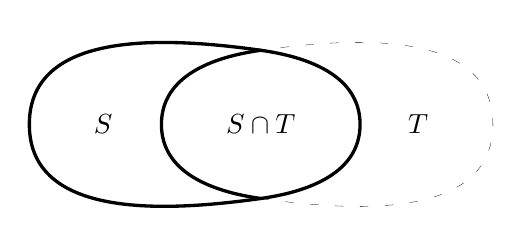
\begin{tikzpicture}[very thick]

\begin{scope}[every node/.style={inner sep=.8cm}]
\node(s) at(-2,0) {$S$};
\node(st) at(0,0) {$S \cap T$};
\node(t) at(2,0) {$T$};
\end{scope}

\draw 
(s.west) to[out=90, in=172] 
(st.north) to[out=-8, in=90] 
(st.east) to[out=270, in=8]
(st.south) to[out=188, in=270]
(s.west)
;

\draw[outline] 
(st.south) to[out=-8, in=270]
(t.east) to[out=90, in=8] 
(st.north) 
;
\draw 
(st.north) to[out=188, in=90] 
(st.west) to[out=270, in=172]
(st.south)
;

\begin{scope}[->]
\os
\capst
\cupst
\tst
\end{scope}

\end{tikzpicture}
\caption{}
\label{sub:s}
\end{subfigure}
%
%
\begin{subfigure}{.48\linewidth}
\centering
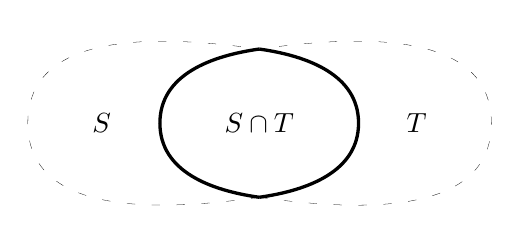
\begin{tikzpicture}[very thick]

\begin{scope}[every node/.style={inner sep=.8cm}]
\node(s) at(-2,0) {$S$};
\node(st) at(0,0) {$S \cap T$};
\node(t) at(2,0) {$T$};
\end{scope}

\draw[outline] 
(st.south) to[out=188, in=270]
(s.west) to[out=90, in=172] 
(st.north)
;
\draw 
(st.north) to[out=-8, in=90] 
(st.east) to[out=270, in=8]
(st.south)
;

\draw[outline] 
(st.south) to[out=-8, in=270]
(t.east) to[out=90, in=8] 
(st.north)
;
\draw 
(st.north) to[out=188, in=90] 
(st.west) to[out=270, in=172]
(st.south)
;

\begin{scope}[->]
\sst
\capst
\tst
\end{scope}

\end{tikzpicture}
\caption{}
\label{sub:cap}
\end{subfigure}
%
\hfill
%
\begin{subfigure}{.48\linewidth}
\centering
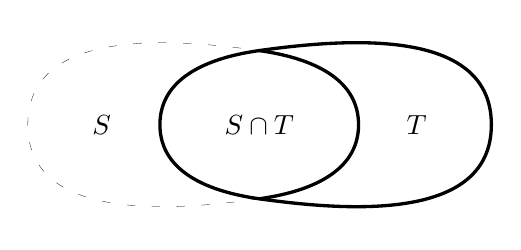
\begin{tikzpicture}[very thick]

\begin{scope}[every node/.style={inner sep=.8cm}]
\node(s) at(-2,0) {$S$};
\node(st) at(0,0) {$S \cap T$};
\node(t) at(2,0) {$T$};
\end{scope}

\draw[outline] 
(st.south) to[out=188, in=270]
(s.west) to[out=90, in=172] 
(st.north)
;
\draw 
(st.north) to[out=-8, in=90] 
(st.east) to[out=270, in=8]
(st.south)
;

\draw 
(t.east) to[out=90, in=8] 
(st.north) to[out=188, in=90] 
(st.west) to[out=270, in=172]
(st.south) to[out=-8, in=270]
(t.east)
;

\begin{scope}[->]
\sst
\cupst
\ot
\end{scope}

\end{tikzpicture}
\caption{}
\label{sub:t}
\end{subfigure}
%
\caption[]{%
Given the two solutions on the left, 
\subref{sub:cup} and \subref{sub:cap}, we
can construct the two solutions on the right side,
\subref{sub:s} and \subref{sub:t}, with equal total weight.
The edges of type 
\inlineedge{e1}, 
\inlineedge{e2}, 
\inlineedge{e3}, 
\inlineedge{e6}
from the left side are ``naturally'' distributed over the two solutions on the
right side and the edges of type \inlineedge{e5} and \inlineedge{e4} can be
distributed between the two solutions without violating the capacity constraints.
}
\label{fig:sub}
\end{figure}


Buchbinder et al.~\cite{BFNS15,buchbinder2016deterministic} presented
a general $\half$-approximation algorithm for unconstrained
submodular maximization, thus we have the following theorem.

\begin{theorem}
There exists a polynomial time $\half$-approximation algorithm
for \carpool.
\end{theorem}


Now consider \gcp.  Recall that in this variant of \carpool, in
addition to the capacity function $c:V \to \N$, and the weight
function $w:A \to \R^+$, we are also given a size function $s:V \to
\N$, and the constraint $\din[M](v) \leq c(v)$ is replaced with the
constraint $\sum_{u:(u,v) \in M} s(u) \leq c(v)$.
%
%The motivation for this variant of the problem is when we want to
%allow a group of people to travel together in the same car, thus $s$
%is the size of the group.
%
We show that this variant of the problem does not fit the submodular
maximization formulation as defined for \carpool.
%
Recall the submodular maximization formulation given above,
%in Section~\ref{sec:sub},
namely $\barw: 2^V \to \R$, where $\barw(S)
\eqdf w(M(S))$ and $M(S)$ is the maximum weight carpool matching that
satisfies $D_{M(S)} \subseteq S \subseteq V \setminus P_{M(S)}$.
%
Figure~\ref{fig:not submodular} contains an instance that shows that
the function $\barw$ is not submodular anymore.

\begin{figure}[!t]
\begin{center}
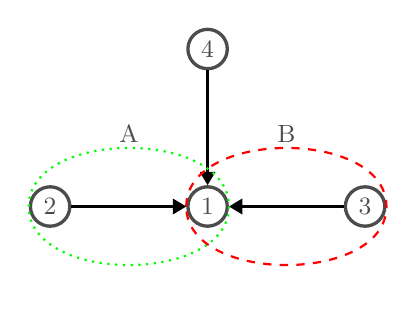
\begin{tikzpicture}[every node/.style={default node},thick]

\node(1) at (-2,0){2};
\node(2) at (0,0){1};
\node(3) at (2,0){3};
\node(4) at (0,2){4};

\draw[->] (1) -- (2);
\draw[->] (3) -- (2);
\draw[->] (4) -- (2);

\draw[dotted,green] 
(1.west) to[out=90,in=90] node[label above] {A}
(2.east) to[out=-90, in=-90]
(1.west)
;

\draw[dashed,red] 
(2.west) to[out=90,in=90] node[label above] {B}
(3.east) to[out=-90, in=-90]
(2.west)
;
\end{tikzpicture}
\end{center}
\caption{An unweighted \carpool instance: $c(1) = 2$, $s(2) = s(3) =
  1$, and $s(4) = 2$.  We have that $\barw(A) + \barw(B) = 2 < 3 =
  \barw(A \cup B) + \barw(A \cap B)$.}
\label{fig:not submodular}
\end{figure}


%%%%%

\subsection{A Star Improvement Algorithm}
\label{sec:improve}

In this section we give a local search $(\half-\eps)$-approximation
algorithm for \carpool.  This algorithm repeatedly checks whether the
current carpool matching $M$ can be improved by means of a star
centered at a vertex $v$.  The profit from this star is the total
weight of the arcs in the star, and the cost is the total weight of
lost arcs (e.g., arcs from passengers to drivers that became
passengers of $v$).  If the profit is larger than the cost, then an
improvement step is performed.  The algorithm terminates when such a
step is not possible.
%
At the end of the section we show that this algorithm extends to \gcp.

%We remind the reader that this algorithm will be extended to \gcp in
%Section~\ref{sec:group}.

We need a few definitions before presenting our algorithm.
%
Given a directed graph $G = (V,A)$, define $\nin[](v) \eqdf \set{u :
  (u,v) \in A}$ and $\nout[](v) \eqdf \set{u : (v,u) \in A}$.
%
Given a feasible carpool matching $M$, the weight $w_M(v)$ of a vertex
$v$ with respect to $M$ is the sum of the weights of the arcs in $M$
that are incident on $v$, namely
\[
w_M(v)
\eqdf w(M \cap \nin[](v)) + w(M \cap \nout[](v))
=     \sum_{(u, v) \in M} w(u, v) + \sum_{(v, u) \in M} w(v, u)
~.
\]
For a subset of vertices $U \subseteq V$ we define
$w_M(U) \eqdf \sum_{v \in U} w_M(v)$.

We now argue that, with respect to any carpool matching $M$, the total
weight of all the vertices is equal to twice the weight of the matching.

\begin{observation}
\label{lm:val-twice}
$w_M(V) = 2 w(M)$.
%\sum_{v \in V} w_M(v) = 2 \sum_{e \in M} w(e)$.
\end{observation}
\begin{proof}
%We have that 
\(\displaystyle
w_M(V)
= \sum_{v \in V} w_M(v)
= \sum_{v \in V} \sum_{(u, v) \in M} w(u, v) +
    \sum_{v \in V} \sum_{(v, u) \in M} w(v, u) 
= 2 \sum_{e \in M} w(e)
%~.    
\).
\end{proof}

Denote by $\delta_M(u,v)$ the difference between the weight of the arc
and the weight of its source vertex, that is:
\[
\delta_M(u, v) \eqdf w(u, v) - w_M(u)
~.
\]
For a subset $S \subseteq A$ of arcs define
$\delta_M(S) \eqdf \sum_{(u,v) \in S} \delta_M(u,v)$.

A subset $S_v$ of arcs entering a vertex $v$, whose size is not
greater than the capacity of $v$, is called an \emph{improvement} to
vertex $v$ if $\delta(S_v)$ is greater than the value of $v$.  More
formally, 

\begin{definition}
A subset $S_v \subseteq A \cap (V \times \{v\})$ is
an \emph{improvement} with respect to a carpool matching $M$, if
%the following conditions hold:%
\begin{inparaenum}[(i)]
\item $\abs{S_v} \leq c(v)$, and
\item $\delta_M(S_v) > w_M(v)$.
\end{inparaenum}
Furthermore, if there exists an improvement for a vertex $v$, we say
that vertex $v$ can be \emph{improved}.
\end{definition}

Given an arc $(u,v) \in A$, let $\inc(u,v)$ be the set of arcs that
are incident on $(u,v)$, namely define
\[
\inc(u,v)
\eqdf (\nin[](u) \times \{u\}) \cup (\{u\} \times \nout[](u)) \cup
      (\nin[](v) \times \{v\}) \cup (\{v\} \times \nout[](v))
~.
\]
If $S$ is a set of arcs, then $\inc(S) \eqdf \bigcup_{(u,v) \in
S} \inc(u,v)$.
%
Figure~\ref{fig:defs} depicts all the above definitions.

\begin{figure}[t]
\centering
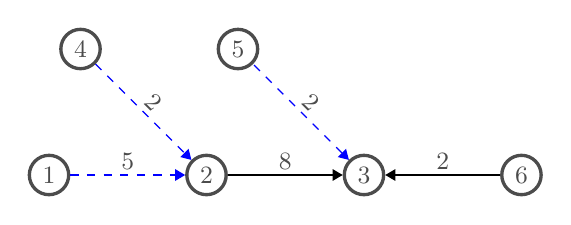
\begin{tikzpicture}[every node/.style={default node}]

\node(1) at(0,0) {1};
\node(2) at(2,0) {2};
\node(3) at(4,0) {3};

\node(4) at(.4,1.6) {4};
\node(5) at(2.4,1.6) {5};
\node(6) at(6, 0) {6};

\draw[m,->] (1) -- (2) node[label above]{$5$};
\draw[m,->] (4) -- (2) node[label above]{$2$};
\draw[m,<-] (3) -- (5) node[label above]{$2$};
\draw[->] (6) -- (3) node[label above]{$2$};
\draw[->] (2) -- (3) node[label above]{$8$};

\end{tikzpicture}
\caption{In this example $M$ is the set of the blue, dashed arcs.
In this case $w_M(2) = 7$, $w_M(5) = 2$, and $w_M(6) = 0$.  Also,
$\delta_M(2, 3) = 1$ and $\delta_M(6, 3) = 2$.  The set $\set{(2,3),
(6,3)}$ is an \emph{improvement} to vertex 3 and $\inc(2,3)
= \set{(1,2),(4,2),(3,5),(6,3)}$.}
\label{fig:defs}
\end{figure}

We are now ready to describe our local search algorithm, which is
called \textbf{StarImprove} (Algorithm~\ref{alg:grd}).  It starts with
an empty carpool matching $M$, and in every iteration it looks for a
vertex that can be improved.  If there exists such a vertex $v$, then
the algorithm removes the arcs that are incident on $S_v$ from $M$,
and adds the arcs in $S_v$.  The algorithm terminates when no vertex
can be improved.  Figure~\ref{fig:improvement} depicts an improvement
step.

\begin{algorithm}
\caption{\textbf{StarImprove}$(G,c)$}
\label{alg:grd}
%\begin{small}
$M \gets \emptyset$ \\
\Repeat{$\text{done}$}{
	$\text{done} \leftarrow \textsc{True}$ \\
	\For{$v \in V$}{
		\If{there exists an improvement $S_v$}{
			$M \leftarrow M \setminus \inc(S_v) \cup S_v$	\\
			$\text{done} \leftarrow \textsc{False}$ \\
		}
	}
}
%\end{small}
\end{algorithm}

\begin{figure}[t]
\centering
\begin{subfigure}{.4\linewidth}
\centering
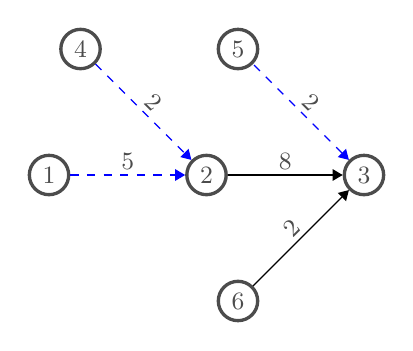
\begin{tikzpicture}[every node/.style={default node}]
\node(1) at(0,0) {1};
\node(2) at(2,0) {2};
\node(3) at(4,0) {3};

\node(4) at(.4,1.6) {4};
\node(5) at(2.4,1.6) {5};
\node(6) at(2.4, -1.6) {6};

\draw[m,->] (1) -- (2) node[label above]{$5$};
\draw[m,->] (4) -- (2) node[label above]{$2$};
\draw[m,<-] (3) -- (5) node[label above]{$2$};
\draw[->] (6) -- (3) node[label above]{$2$};
\draw[->] (2) -- (3) node[label above]{$8$};

\end{tikzpicture}
\caption{A matching that can be improved.}
\end{subfigure}
%
\hfill
%
\begin{subfigure}{.5\linewidth}
\centering
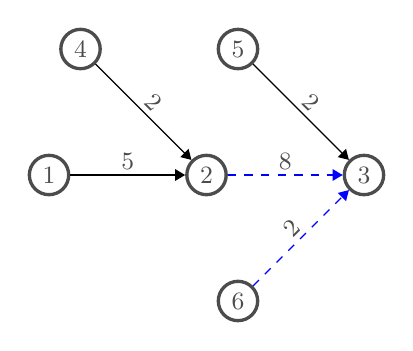
\begin{tikzpicture}[every node/.style={default node}]
\node(1) at(0,0) {1};
\node(2) at(2,0) {2};
\node(3) at(4,0) {3};

\node(4) at(.4,1.6) {4};
\node(5) at(2.4,1.6) {5};
\node(6) at(2.4, -1.6) {6};

\draw[->] (1) -- (2) node[label above]{$5$};
\draw[->] (4) -- (2) node[label above]{$2$};
\draw[<-] (3) -- (5) node[label above]{$2$};
\draw[m,->] (6) -- (3) node[label above]{$2$};
\draw[m,->] (2) -- (3) node[label above]{$8$};

\end{tikzpicture}
\caption{The matching after improving vertex 3.}
\end{subfigure}
\caption{An improvement example.}
\label{fig:improvement}
\end{figure}

We proceed to bound the approximation ratio of the algorithm, assuming
termination.

For a vertex $v$ and a set $S$ of edges entering $v$, let $\nin[S](v)
= \set{u : (u,v) \in S}$ be the set in-neighbors corresponding to $S$.

\begin{lemma}
\label{lm:no improve}
Let $M$ be a matching computed by \textbf{StarImprove}.  Let $v$ be a
vertex with no improvement, and let $S \subseteq \nin(v)$, such that
$\abs{S} \leq c(v)$, then $w(S) \leq w_M(v) + w_M(\nin[S](v))$.
\end{lemma}
\begin{proof}
If no improvement exists, then we have that 
\[
w(S) - w_M(\nin[S](v))
=    \sum_{(u,v) \in S} (w(u,v) - w_M(u))
=    \delta_M(S) 
\leq w_M(v)
~,
\]
as required.
\end{proof}

To bound the approximation ratio of the algorithm, we use a charging
scheme argument.

\begin{lemma}
If \textbf{StarImprove} terminates, then the computed solution is
$\half$-approximate.
\end{lemma}
\begin{proof}
Let $M$ be the matching produced by the algorithm, and let $M^*$ be an
optimal matching.  We load every vertex $v$ with an amount of money
equal to $w_M(v)$, and then we show that this is enough to pay for
every arc in the optimal matching.  Due to
Observation~\ref{lm:val-twice} the total amount of money that we use
is exactly twice the weight of $M$.

Consider a driver $v \in D_{M^*}$, and let $S = (V \times \{v\}) \cap
M^*$.  By lemma~\ref{lm:no improve} we know that $w(S) \leq w_M(v) +
w_M(\nin[S](v))$, thus we can pay for $S$, using the money on $v$ and
on $\nin[S](v)$.  These vertices are not charged again, since the
stars are disjoint in $M^*$.
\end{proof}

We show that our analysis is tight using Figure~\ref{fig:grd worst}.

\begin{figure}[t]
\centering
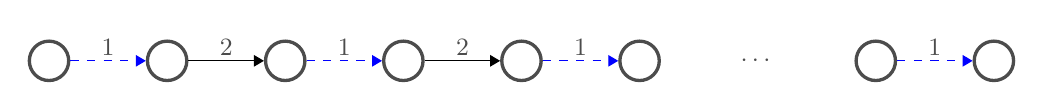
\begin{tikzpicture}[every node/.style={default node}, ->]

\def\sep{1.5}

\foreach \n in {0,...,5}{
	\pgfmathsetmacro{\x}{\n * \sep}
	\node(\n) at(\x,0){};
}

\foreach \n/\m in {0/1,2/3,4/5}{
	\draw[m] (\n) -- (\m) node[label above]{1};
}

\foreach \n/\m in {1/2,3/4}{
	\draw[] (\n) -- (\m) node[label above]{2};
}

\pgfmathsetmacro{\x}{6 * \sep}
\node[draw=none] at(\x, 0){$\cdots$};

\foreach \n in {7,...,8}{
	\pgfmathsetmacro{\x}{\n * \sep}
	\node(\n) at(\x,0){};
}

\draw[m] (7) -- (8) node[label above]{1};


\end{tikzpicture}
\caption{
%
Consider a directed path with $n$ vertices and $(n-1)$ arcs, where $n$
is even.  The weights for the arcs are alternating between 1 and 2.
%
If \textbf{StarImprove} selects all arcs of weight 1, then no further
improvement can be done and the value of the matching is $n/2$,
while the optimal matching has value of $n-2$.}
\label{fig:grd worst}
\end{figure}

It remains to consider the running time of the algorithm.

\begin{theorem}
\label{thm:improve-bounded}
Algorithm~\textbf{StarImprove} is a $\half$-approximation algorithm
for \carpool, if edge weights are integral and polynomially bounded.
\end{theorem}
\begin{proof}
First, observe that determining if a vertex $v$ can be improved can be
done efficiently by considering the incoming arcs to $v$ in a
non-increasing order of their $\delta_M$s, and only ones with positive
values.  A vertex $v$ can be improved, then, if the $\delta_M$s of the
first $c(v)$ (or less) arcs sum up to more than $w_M(v)$.
%
It follows that the running time of an iteration of the for-loop is
polynomial.  Since the edge weights are integral and polynomially
bounded, the weight of an optimal carpool matching is polynomially
bounded.  The algorithm runs in polynomial time, because in each
iteration the algorithm improves the weight of the matching by at
least one or otherwise it terminates.
\end{proof}

%%%%%

Next we show that \gcp has a $(\half -\eps)$-approximation algorithm
by extending Algorithm~\textbf{StarImprove}.
%the local improvement algorithm from Section~\ref{sec:improve}.
%

%
This leads to the following result.

\begin{theorem}
Algorithm~\textbf{StarImprove} is a $\half$-approximation algorithm
for \gcp, if edge weights are integral and polynomially bounded.
\end{theorem}
\begin{proof}
The main concern when trying to adopt the algorithm to \gcp is how to
efficiently determine whether a vertex can be improved.
%
With \carpool, if weights are polynomially-bounded, it was enough to
consider the incoming arcs to a vertex $v$ in a non-increasing order
of $\delta_M$ (see proof of Theorem~\ref{thm:improve-bounded}).  This
does not work anymore, since in the \gcp we have sizes.  In fact,
given $v$, finding the best star with respect to $\delta_M$ is a
\textsc{Knapsack} instance where the size of the knapsack is $c(v)$.
%
If weights are polynomially-bounded, then $\delta_M(e)$ is bounded for
every arc $e \in A$, and therefore this instance of \textsc{Knapsack}
can be solved in polynomial time using dynamic programming.
%
As before, the number of improvements is polynomial, since the weight
of an optimal solution is polynomially bounded.
\end{proof}

%%%%%

It remains to consider the case, where weights are not polynomially
bounded.  We prove that one can use standard scaling and rounding to
ensure a polynomial running time in the cost of a slight degradation
of the approximation ratio.

\begin{theorem}
\label{thm:improve}
There exists a $(\half-\eps)$-approximation algorithm for \carpool (or
\gcp), for every $\eps \in (0,\half)$.
\end{theorem}
\begin{proof}%[Proof of Theorem~\ref{thm:improve}]
Define the weight function $w'(e)
= \floor{\frac{w(e)}{w_{\max}} \cdot \frac{m}{2\eps}}$, where
$w_{\max} \eqdf \max_{e \in A} w(v)$.
%
Let $M^*$ and $M'$ be an optimal carpool matching with respect to $w$
and $w'$, resp.  We have that
\[
w'(M^*)
=    \sum_{e \in M^*} \floor{\frac{w(e)}{w_{\max}} \cdot \frac{m}{2\eps}}
>    \sum_{e \in M^*} \paren{ \frac{w(e)}{w_{\max}} \cdot \frac{m}{2\eps} } - m
=    \frac{m}{2\eps w_{\max}} \cdot w(M^*) - m
~.
\]
Since $w(M^*) \geq w_{\max}$, we have that 
\[
w'(M^*)
>    \frac{m}{2\eps w_{\max}} \cdot (w(M^*) - 2\eps w_{\max})
\geq \frac{m}{2\eps w_{\max}} \cdot (1 - 2\eps) w(M^*)
~.
\]
By Theorem~\ref{thm:improve-bounded}, our local improvement algorithm
computes a $\half$-approximate carpool matching $M$ on $(G, c, w')$,
and this matching satisfies $w'(M) \geq w'(M')/2$.  Furthermore, since
$w'(M') \geq w'(M^*)$, it follows that $w'(M) \geq w'(M^*)/2$.
Therefore
\[
w(M)
\geq \frac{2\eps w_{\max}}{m} w'(M) 
\geq \frac{1}{2} \frac{2\eps w_{\max}}{m} w'(M^*)
>    \frac{1-2\eps}{2} w(M^*)
~,
\]
as required.
\end{proof}

%Using standard scaling and rounding we obtain the following result.

%\begin{theorem}
%There exists a $(\half-\eps)$-approximation algorithm for \gcp,
%for every $\eps \in (0,\half)$.
%\end{theorem}



%%%%%%%%%%%%%%%%%%%%%%%%%%%%%%%%%%%%%%%%%%%%%%%%%%%%%%%%%%%%%%%%%%%%%%%%%

\section{Constant Maximum Capacity}
\label{sec:cmax}

In this section we study the \carpool problem when the maximum
capacity is constant, i.e., when $\cmax = O(1)$.  We show that this
variant of the problem is APX-hard even for unweighted and undirected
instances.  We also describe and analyze a local search algorithm for
the unweighted variant of the problem and show that the algorithm
achieves a $\half + \inv{2\cmax} - \eps$ approximation ratio, for any
$\varepsilon > 0$.
%
This algorithm also applies to \gcp.

%%%%%

\subsection{Hardness}
\label{sec:hardness}

As we mentioned earlier, \textsc{Spanning Star Forest} has a lower
bound of $\frac{10}{11} + \eps$ for any $\eps > 0$, unless
P$=$NP~\cite{ChakrabartyGoel10}, and this bound applies to \carpool.
%
The result, however, does not hold for the case where $\Delta = O(1)$
(and $\cmax = O(1)$).  In this section we show that the problem remains
APX-hard even in this case.

Formally, the (unweighted) \textsc{Minimum Dominating Set} problem is
defined as follows.  The input is an undirected graph $G = (V,E)$, and
a feasible solution, or a \emph{dominating set}, is a subset
$D \subseteq V$ that dominates $V$ namely such that
$D \cup \bigcup_{v \in D} N(v) = V$, where $N(v)$ is the neighborhood
of $v$.  The goal is to find a minimum cardinality dominating set.
%
\textsc{Minimum Dominating Set-$b$} is the special case of
\textsc{Minimum Dominating Set} in which
the maximum degree of a vertex in the input graph $G$ is bounded by
$b$.  The problem was shown to be APX-hard, for $b \geq 3$, by
Papadimitriou and Yannakakis~\cite{PapYan88}.

We now consider the unweighted and undirected special case of
the \carpool problem.  In this case, the input consists of an
undirected graph $G$ and a capacity function $c$, and the goal is to
find a carpool matching $M$ that maximizes $\abs{P_M}$.

Given an undirected graph $G$, let $D^*$ be a minimum cardinality
dominating set, and let $M^*$ be an optimal carpool matching with
respect to $G$ and the capacity function: $c(v) = \deg(v)$, for every
$v \in V$.

\begin{observation}
$\abs{P_{M^*}} + \abs{D^*} = \abs{V}$ 
\end{observation}
\begin{proof}
Given a carpool matching $M$, observe that $D_M \cup Z_M$ is a
dominating set.  In the other direction, a dominating set $D$ induces
a carpool matching of size $\abs{V \setminus D}$.
\end{proof}

We use this duality to obtain a hardness result for \carpool.

\begin{theorem}
The \carpool problem is APX-hard, even for undirected and unweighted
instances with maximum degree bounded by $b$, for $b \geq 3$.
\end{theorem}
\begin{proof}
We prove the theorem by presenting an $L$-reduction from
\textsc{Minimum Dominating Set-$b$}.
(For details on $L$-reductions the reader is referred to~\cite{PapYan88}.)
%
We define a function $f$ from \textsc{Minimum Dominating Set-$b$}
instances to \carpool instances as follows: $f(G) = (G,c)$, where
$c(v) = \deg(v)$, for every $v \in V$.  Next, we define a function $g$
that given a carpool matching computes a dominating set as follows:
$g(M) = V \setminus P_{M}$.  Both $f$ and $g$ can be computed in
polynomial time.

Let $D^*$ be an optimal dominating set with respect to $G$, and let
$M^*$ be an optimal carpool matching with respect to $G$ and $c$.
Since $|D^*| \geq \frac{|V|}{b+1}$, it follows that 
\(
\abs{P_{M^*}} \leq b \abs{D^*}
%~,
\),
In addition, if $M$ is a carpool matching, we have that
\[
\abs{D_M \cup Z_M} - \abs{D^*}
= (\abs{V} - \abs{P_M}) - \abs{D^*}
= \abs{P_{M^*}} - \abs{P_M}
~.
\]
Hence, there is an $L$-reduction from \textsc{Minimum Dominating
Set-$b$} to unweighted and undirected \carpool with bounded capacity
$b$.
\end{proof}

%%%%%

\subsection{Local Search}
\label{sec:local}

In this section we present a local search $(\half + \inv{2c_{\max}} -
\eps)$-approximation algorithm for unweighted \carpool whose running
time is polynomial if $c_{\max} = O(1)$.

Let $k$ be a constant integer to be determined later.
Algorithm~\textbf{EdgeSwap} (Algorithm~\ref{alg:local}) maintains a
feasible matching $M$ throughout its execution and operates in
iterative manner where in each iteration it tries to find a better
solution by replacing a subset of at most $k$ edges in the current
solution with another (larger) subset of edges not in the solution.
The algorithm halts when no improvement can be done. 

\begin{algorithm}
\caption{\textbf{EdgeSwap}$(G,c,k)$}
\label{alg:local}
%\begin{small}
\SetKw{True}{true}
\SetKw{False}{false}
%\KwIn{$G = (V, A)$, $c : V \rightarrow \N$, $k$}
%\KwOut{$M$}
$M \leftarrow \emptyset$								\\
\Repeat{done}{
 	$done \leftarrow{}$ \True							\\
 	\ForAll{$M' \subseteq M : |M'| \leq k$}{
 		\ForAll{$A' \subseteq A \setminus M : |A'| = |M'| + 1$}{
			\If{$M \setminus M' \cup A'$ is feasible}{
				$M \leftarrow{} M \setminus M' \cup A'$	\\
				$done \leftarrow{}$ \False				\\
			}
		}
 	}
}
\Return{$M$}
%\end{small}
\end{algorithm}

Algorithm~\textbf{EdgeSwap} terminates in polynomial time, since in
every non-final iteration it improves the value of the solution by
one.  Thus, after at most $n$ iterations the algorithm terminates.  In
every iteration the algorithm examines all subsets of edges of a fixed
size and tests for feasibility, both these operations can be done in
polynomial time.

Observe that a vertex $v \in D_M \cup Z_M$ is the center of a
\emph{directed star} whose leaves are the passengers in the set
$P_M(v) = \set{u : (u,v) \in M}$.  Observe that $P_M(v) = \emptyset$,
for $v \in Z_M$ (in this case the star is an isolated vertex).
%
Given a carpool matching $M$, we define $\calS(M)$ to be the set of
stars that are induced by $M$.
%
Denote by $V(S)$ the set of vertices of a star, i.e., if $v$ is the
center of $S$, then $V(S) = \{v\} \cup P_M(v)$.  
Also, let $A(S)$ be
the arcs of $S$.
%
Observe that $V(S) = \{v\}$ and $A(S) = \emptyset$, if $v \in Z_M$.
%
For $\calT \subseteq \calS(M)$, define $V(\calT) \eqdf \bigcup_{S \in
  \calT} V(S)$ and $A(\calT) \eqdf \bigcup_{S \in \calT} A(S)$.

It remains to analyze the approximation ratio of \textbf{EdgeSwap}.
Consider an optimal matching $M^*$, and $M$ be the matching computed
by \textbf{EdgeSwap}.  Given both matchings we build the \emph{star
  graph} of the two solutions in which each vertex represents a star
from the optimal solution, namely from $\calS(M^*)$, and an edge
exists between two vertices if there is a star in $\calS(M)$ that
intersects the two corresponding stars of the optimal solution.
%
Formally we defined an undirected \emph{star graph} $\calH =
(\calS(M^*), \calE)$, where
\[
\calE = \set{(S^*_i, S^*_j) : \exists S \in \calS(M), 
             V(S) \cap V(S^*_i) \neq \emptyset \land
             V(S) \cap V(S^*_j) \neq \emptyset}
~.
\]
Figure~\ref{fig:conflict} depicts a star graph.



\begin{figure}[t]
%\centering
%
\begin{subfigure}[b]{.47\linewidth}
\centering
\newcommand{\edge}[2]{
	\draw (#1) -- (#2);
}

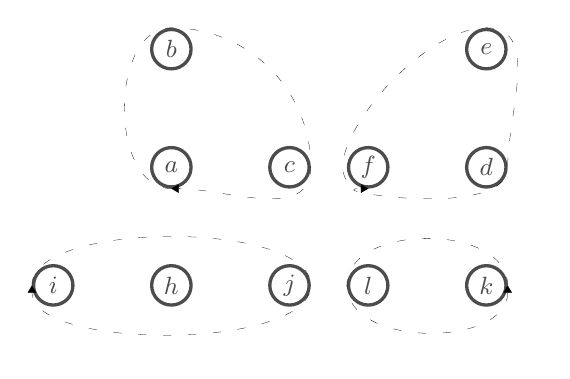
\begin{tikzpicture}[every node/.style={default node}, ->, very thick]

\node(1) at(0,0) {$a$};
\node(2) at(0,1.5) {$b$};
\node(3) at(1.5,0) {$c$};

\node(4) at(4,0) {$d$};
\node(5) at(4,1.5) {$e$};
\node(6) at(2.5,0) {$f$};

\node(7) at(0,-1.5) {$h$};
\node(8) at(-1.5,-1.5) {$i$};
\node(9) at(1.5,-1.5) {$j$};

\node(10) at(4,-1.5) {$k$};
\node(11) at(2.5,-1.5) {$l$};

\draw[outline]
(1.south) to[out=180,in=180] 
(2.north) to[out=0,in=90]
(3.east) to[out=-90,in=0]
(1.south)
;

\draw[outline]
(8.west) to[out=90,in=90,looseness=.6] 
(9.east) to[out=-90,in=-90,looseness=.6]
(8.west)
;

\draw[outline]
(6.south) to[out=180,in=180] 
(5.north) to[out=0,in=90]
(4.east) to[out=-90,in=180]
(6.south)  
;

\draw[outline]
(10.east) to[out=90,in=90] 
(11.west) to[out=-90,in=-90]
(10.east)  
;

\begin{scope}[dashed, red]
\edge{2}{1}
\edge{3}{1}

\edge{5}{4}
\edge{6}{4}

\edge{8}{7}
\edge{9}{7}

\edge{11}{10}
\end{scope}

\begin{scope}[green]
\edge{2}{5}

\edge{7}{1}
\edge{3}{9}
\end{scope}

\end{tikzpicture}
\caption{$M^*$ is depicted by the dashed red edges,
and $M$ is depicted by the solid green edges.
The optimal stars are outlined.
}
\end{subfigure}
%
\hfill
%
\begin{subfigure}[b]{.51\linewidth}
\centering
\newcommand{\edge}[2]{
	\draw (#1) -- (#2);
}

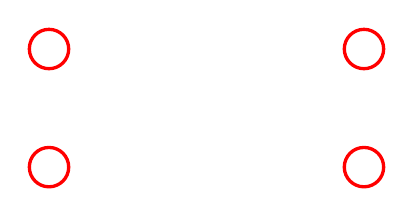
\begin{tikzpicture}[every node/.style={default node, red}, -, very thick, green]

\node(1) at(0,0) {};
\node(2) at(4,0) {};
\node(3) at(0,-1.5) {};
\node(4) at(4,-1.5) {};

\edge{1}{2}
\edge{1}{3}

\end{tikzpicture}
\vspace{25pt}
\caption{The star graph $\calH$: each vertex corresponds to a star in
  $G$ which is induced by $M^*$.  The upper left vertex of $\calH$
  corresponds to the star in $G$ containing $a$, $b$, and $c$.}
\end{subfigure}
%
\caption{An example of a star graph $\calH$.}
\label{fig:conflict}
\end{figure}

\begin{lemma}
\label{lemma:maxdegH}
The maximum degree of $\calH$ is $\cmax(\cmax+1)$.
\end{lemma}
\begin{proof}
Each star in $\calS(M^*)$ contains at most $\cmax+1$ vertices and each
such vertex can belong to a star in $\calS(M)$ containing additional
$\cmax$ vertices, each of which is located in a different star in
$\calS(M^*)$.
\end{proof}

In what follows we compare $\abs{M}$ and $\abs{M^*}$ in maximal
connected components of the star graph $\calH$.  Intuitively, we show
that $M$ is optimal on small maximal components, and that the
approximation ratio on medium (non-necessarily) components can be
bounded due to the termination condition of \textbf{EdgeSwap}.  Large
maximal components will be partitioned into medium components.

We first show that large connected graphs (or maximal connected
components) can be partitioned into medium size components.
%The proof is omitted for lack of space.
%The proof is given in Appnedix~\ref{sec:omitted}.

\begin{lemma}
\label{lemma:dec}
An undirected connected graph $G = (V,E)$ with maximum degree
$\Delta$, can be decomposed into connected components of size at least
$\ell$ and at most $\Delta \ell$, if $\ell \leq \abs{V}$.
\end{lemma}
\begin{proof}%[Proof of Lemma~\ref{lemma:dec}]
We give a constructive proof.
%
First, if $\ell \leq |V| \leq \Delta \ell$, then we are done.
%
Otherwise, we partition the graph recursively as follows.  Let $U
= \emptyset$.  As long as $\abs{U} < \ell$, choose an arbitrary vertex
$u$ such that $U \cup \set{u}$ is connected and add $u$ to $U$.
%
If the graph $G[V \setminus U]$, which is induced by $V \setminus U$,
is connected, then choose the next vertex.
%
However, if $G[V \setminus U]$ becomes disconnected, then consider the
maximal connected components of $G[V \setminus U]$.  Add the vertices
of any maximal component that contains less than $\ell$ vertices to
$U$.  Observe that afterwards $\abs{U} < \ell + (\Delta-1) \ell
= \Delta \ell$.
%
If $\abs{U} \geq \ell$, then recursively partition any component of
$G[V \setminus U]$ that contains more than $\ell$ vertices.
%
If $\abs{U} < \ell$, then there must exist at least one maximal
component $C$ of $G[V \setminus U]$ that contains more than $\ell$
vertices.  In this case recursively partition any maximal component of
$G[V \setminus (U \cup C)]$ that contains more than $\ell$ vertices.
Also, continue to augment $U$ in the graph $G[U \cup C]$.
\end{proof}

\iffalse %%%%%% Removed

\begin{proof}
Let $T$ be any spanning tree of $G$ and let $r$ be an arbitrary root.
Starting with $r$, repeatedly choose a child whose subtree is strictly
larger than $\frac{\Delta-1}{\Delta} \abs{V}$, until this is not
possible.  Hence, we have reached a vertex $v$ whose subtree contains
more than $\frac{\Delta-1}{\Delta} \abs{V}$ vertices, but the subtrees
of its children contain at most $\frac{\Delta-1}{\Delta} \abs{V}$
vertices.
%
If $v = r$, then $v$ has a child $u$ with at least $\inv{\Delta}
(\abs{V}-1) \geq \ell$ vertices.  Otherwise, there exists a child $u$
of $v$ whose subtree is of size at least
$\inv{\Delta} \abs{V} \geq \ell$.  Disconnect $u$ and the vertices in
its subtree from the graph.
%
In both cases $u$'s subtree contains at most
$\frac{\Delta-1}{\Delta} \abs{V}$ vertices, and thus at least
$\inv{\Delta} \abs{V} \geq \ell$ vertices remain in the graph.  Hence
we obtain two connected subgraphs of size at least $\ell$.
%
We repeat this procedure recursively on any component of size
strictly larger $\Delta\ell$.
\end{proof}

\fi %%%%%% End removed

Given a carpool matching $M$, define $\deg_M(v) \eqdf \din[M](v) +
\dout[M](v)$.  For a subset $U \subseteq V$ of vertices define
$\deg_M(U) \eqdf \sum_{v \in U} \deg_M(v)$.
%
Observe that $\abs{M} = \half \deg_M(V)$.

In the next lemma we bound the degree ratio in a component that
contains stars with at most $k$ arcs.

\begin{lemma}
\label{lemma:r}
Let $\calT \subseteq \calS(M^*)$ that induces a connected subgraph of
$\calH$.  If $\abs{A(\calT)} \leq k$, then
\[
\frac{\deg_M(V(\calT))}{\deg_{M^*}(V(\calT))} 
\geq \half + \inv{2\cmax} - \inv{2\cmax\abs{\calT}}
~.
\]
\end{lemma}
\begin{proof}
We say that a carpool matching $M$ in $G$ \emph{intersects} $V(\calT)$
if one of the edge in $M$ is incident on one of the vertices in
$V(\calT)$.
%
Consider the solution $M'$ obtained from $M$ by removing all the edges
from $M$ that intersect $V(\calT)$ and adding all the edges from $M^*$
that intersect $V(\calT)$.  Observe that if an edge $(u,v)$ in $M^*$
intersects $V(\calT)$, then $\set{u,v} \in V(\calT)$ by the definition
of the graph $\calH$.  Hence, $M'$ is a feasible carpool matching.

Since $\calT$ induces a connected subgraph of $\calH$, the removal of
edges in $M$ that intersect $V(\calT)$ decreased $\abs{M}$ by at most
$\deg_M(V(\calT)) - \abs{\calT} + 1$.
%
On the other hand, the increase in size is exactly $\half
\deg_{M^*}(V(\calT)) \leq \cmax \abs{\calT}$.
%
Since $\abs{A(\calT)} \leq k$, we know that this difference cannot be
positive, or else, \textbf{EdgeSwap} would not have terminated.  Thus
\[
\half \deg_{M^*}(V(\calT)) \leq \deg_M(V(\calT)) - \abs{\calT} + 1
~,
\]
and so
\[
\frac{\deg_M(V(\calT))}{\deg_{M^*}(V(\calT))}
\geq \half + \frac{\abs{\calT} - 1}{\deg_{M^*}(V(\calT))}
\geq \half + \frac{\abs{\calT} - 1}{2\cmax \abs{\calT}}
=    \half + \inv{2\cmax} - \inv{2\cmax \abs{\calT}}
~,
\]
as required.
\end{proof}


\iffalse %%%%% Removed

\begin{lemma}
%\label{lemma:dec}
Given a parameter $k$, a connected graph $G$ with a maximum degree $d$
can be decomposed into connected components of size at least $k$, and
at most $d(k-1) + 1$.
\end{lemma}

\begin{proof}
We give a constructive proof.  Start constructing a connected
component by adding adjacent vertices one by one to the component and
removing them from the graph.  If at some point, removing a vertex
disconnect the graph, add all the small components (of size less than
$k$) to the constructed component and decompose the large components
(of size at least $k$) recursively.  Note that removing a vertex can
break the graph to at most $d - 1$ additional components.
\end{proof}

\fi %%%%% End removed

It remains to bound the approximation ratio of \textbf{EdgeSwap}.

\begin{lemma}
If $k \geq \cmax$, then $\abs{M} \geq (\half + \inv{2\cmax}
- \frac{\cmax(\cmax+1)}{2k}) \cdot \abs{M^*}$.
\end{lemma}
\begin{proof}
Consider a maximal (with respect to set inclusion) connected component
of the star graph $\calH$ induced by the vertices in $\calT \subseteq
\calS(M^*)$.
%
If $\abs{M \cap A(\calT)} \leq k$, then it must be that $\abs{M \cap
A(\calT)} = \abs{M^* \cap A(\calT)}$, since otherwise $M \cap
A(\calT)$ could be improved.

It remains to consider a maximal component $\calT$ such that $\abs{M
  \cap A(\calT)} > k$.  Since the number of edges in $S \in
\calS(M^*)$ is at most $\cmax$, it must be that $\abs{V(\calT)} >
\frac{k}{\cmax}$.
%
The maximum degree of $\calH$ is $\cmax(\cmax+1)$ by
Lemma~\ref{lemma:maxdegH}, therefore due to Lemma~\ref{lemma:dec}
(with $\ell = \frac{k}{\cmax^2(\cmax+1)}$) we can partition $\calT$
into connected components each of which contains between
$\frac{k}{\cmax^2(\cmax+1)}$ and $\frac{k}{\cmax}$ vertices.
%
Since each such vertex set $\calX$
%is connected and
contains at most $\frac{k}{\cmax}$ stars, it follows that
$\abs{A(\calX)} \leq k$.
%
Due to Lemma~\ref{lemma:r} we have that
\[
\frac{\deg_M(V(\calX))}{\deg_{M^*}(V(\calX))} 
\geq \half + \inv{2\cmax} - \frac{\cmax(\cmax+1)}{2k}
~.
\]
Since $\deg_{M^*}(V(\calT)) = \sum_{\calX} \deg_{M^*}(V(\calX))$ and
$\deg_M(V(\calT)) = \sum_{\calX} \deg_M(V(\calX))$, it follows that
\[
\frac{\deg_M(V(\calT))}{\deg_{M^*}(V(\calT))}
\geq \half + \inv{2\cmax} - \frac{\cmax(\cmax+1)}{2k}
~.
\]
Since the set of maximal components in $\calH$ induces a partition of
$M$, we have that
\[
\abs{M \cap A(\calT)}
\geq \paren{ \half + \inv{2\cmax} -
             \frac{\cmax(\cmax+1)}{2k}} \abs{M^* \cap A(\calT)}
~,
\]
and 
\[
\abs{M}
=    \sum_{\calT} \abs{M \cap A(\calT)}
\geq \paren{ \half + \inv{2\cmax} - \frac{\cmax(\cmax+1)}{2k}}
       \sum_{\calT} \abs{M^* \cap A(\calT)}
=    \abs{M^*}
~.
\]
\end{proof}

By setting $k = \ceil{\cmax(\cmax+1)/2\eps}$, we get the following
result.

\begin{corollary}
\label{cor:local}
There exists a $(\half + \inv{2\cmax} - \eps)$-approximation algorithm
for unweighted \carpool, for every $\eps>0$.
\end{corollary}

%In Appendix~\ref{sec:tight} we show that our analysis is tight.

\iffalse %%%%% Removed 

We now show that Corollary~\ref{cor:local} is tight.  Consider the
example in Figure~\ref{fig:local search tight}, the example is for the
special case when $k = 11$ and $\cmax = 2$ but this example can be
generalized in a straightforward manner.  One can verify that as the
graph in the example grows, the ratio between the optimal solution
and the local search solution approaches $\frac{3}{4}$.

\begin{figure}[t]
\begin{center}
\scalebox{.9}{
\tikzset{local/.style={
green,
dashed,
}}

\tikzset{opt/.style={
red,
solid,
}}

\begin{tikzpicture}[
	every node/.style={default node, solid}, 
	<-,
	level distance=12mm,
	level/.style={sibling distance=100mm/#1},
	level 1/.style={local},
	level 2/.style={opt},
	level 3/.style={local},
	level 4/.style={opt},
	level 5/.style={local},
	level 6/.style={opt},
]

\node{}
child{ node{}
	child { node{}
		child{ node{}
			child{ node{}
				child{ node{}
					child{ node(1){}}
					child{ node(2){}}
				}
			}
			child{ node{}
				child{ node{}
					child{ node(3){}}
					child{ node(4){}}
				}
			}
		}
	}
	child { node{}
		child{ node{}
			child{ node{}
				child{ node{}
					child{ node(5){}}
					child{ node(6){}}
				}
			}
			child{ node{}
				child{ node{}
					child{ node(7){}}
					child{ node(8){}}
				}
			}
		}
	}
};

\begin{scope}[local]
\draw (1) to[bend right] (5);
\draw (2) to[bend right] (6);
\draw (3) to[bend right] (7);
\draw (4) to[bend right] (8);
\end{scope}

\end{tikzpicture}
}
\caption{A tight example for Corollary~\ref{cor:local}. 
The optimal solution is given by the red solid arcs while the local
search solution is given by the green, dashed arcs.  The solution can
be improved by the local search algorithm only if it removes all the
edges.}
\label{fig:local search tight}
\end{center}
\end{figure}

\fi %%%%% End removed

%%%%%%%%%%%%%%%%%%%%%%%%%%%%%%%%%%%%%%%%%%%%%%%%%%%%%%%%%%%%%%%%%%%%%%%%%

%\section{Group Carpool}
%\label{sec:group}

Finally, we show that a variant of Algorithm~\textbf{EdgeSwap} from
Section~\ref{sec:local} can be used to solve \gcp while keeping the
same approximation guarantees. 
%
The only difference is that when checking feasibility of a set of arcs
we do not compare the number of passengers to the capacity of a
driver, but rather compare the total size of the passengers to the
capacity.

\begin{theorem}
There exists a $(\half + \inv{2\cmax} - \eps)$-approximation algorithm
for unweighted \gcp, for every $\eps>0$.
\end{theorem}

%%%%%%%%%%%%%%%%%%%%%%%%%%%%%%%%%%%%%%%%%%%%%%%%%%%%%%%%%%%%%%%%%%%%%%%%%

\subsection*{Acknowledgements.}

We thank David Adjiashvili and Reuven Bar-Yehuda for helpful
discussions.

\bibliographystyle{abbrv}
\bibliography{carpool}

%%%%%%%%%%%%%%%%%%%%%%%%%%%%%%%%%%%%%%%%%%%%%%%%%%%%%%%%%%%%%%%%%%%%%%%%%

\end{document}
